\documentclass[dvisvgm,tikz,border=4pt]{standalone}
\usepackage{amsmath,amssymb}

\usetikzlibrary{arrows.meta,positioning,automata,shapes,shapes.misc,calc,decorations.pathmorphing,decorations.markings,angles,quotes,patterns,mindmap,matrix,knots,hobby,trees}
\tikzset{->-/.style={decoration={markings, mark=at position 0.5 with {\arrow{Stealth}}}, postaction={decorate}}}
\begin{document}
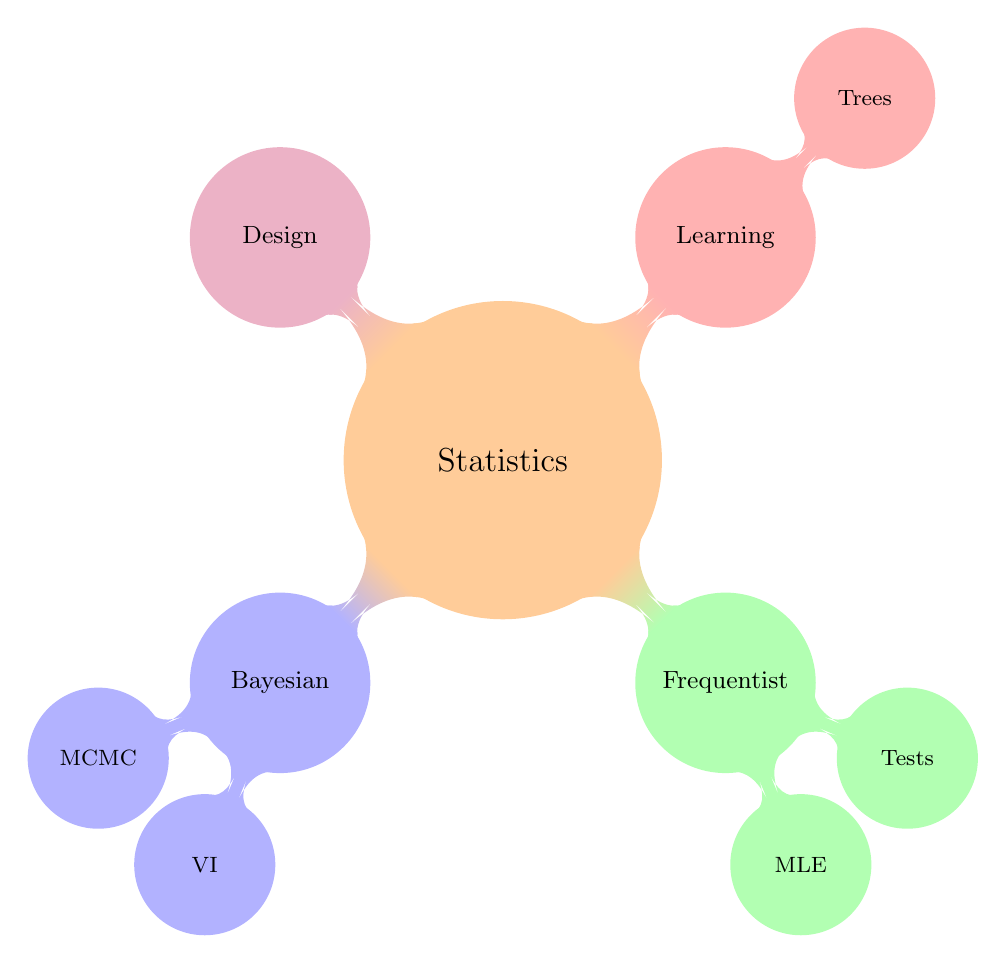
\begin{tikzpicture}[mindmap, grow cyclic, every node/.style=concept, concept color=orange!40, level 1/.append style={level distance=4cm, sibling angle=90}, level 2/.append style={level distance=2.5cm, sibling angle=45}]
\node{Statistics}
  child[concept color=blue!30] { node {Bayesian} child { node {MCMC} } child { node {VI} } }
  child[concept color=green!30] { node {Frequentist} child { node {MLE} } child { node {Tests} } }
  child[concept color=red!30] { node {Learning} child { node {Trees} } }
  child[concept color=purple!30] { node {Design} };
\end{tikzpicture}
\end{document}
